\subsection{\textit{Software} dan \textit{Hardware}}
Pada bagian \textit{software} dan \textit{hardware} akan dijelaskan persyaratan yang dibutuhkan untuk menjalankan aplikasi, mencakup perangkat lunak yang harus diinstal serta spesifikasi perangkat keras yang direkomendasikan untuk kinerja optimal. Berikut ini adalah spesifikasi \textit{software} dan \textit{hardware} yang dibutuhkan untuk menjalankan sistem ini:
\begin{enumerate}
    \item \textit{Software}
    \begin{enumerate}
        \item Sistem operasi \textit{Windows} 10
        \item Web \textit{browser} Chrome.
        \item \textit{Composer}.
        \item IDE (\textit{Integrated Development Environment}) \textit{Visual Studio Code}.
        \item \textit{Database} MySQL.
        \item \textit{Framework} Laravel.   
        \item Git.
        
    \end{enumerate}
    \item \textit{Hardware}
	      \begin{enumerate}
                    \item Prosesor Intel Core i3 atau setara.
    	    	\item RAM (Random Access Memory) 8 GB.
    	      	\item SSD (Solid State Drive) dengan kapasitas 256 GB.
                    \item \textit{Internal/external} GPS (\textit{Global Positioning System}).
                    \item \textit{Webcam}.
    	      	\item \textit{Mouse}.
    	      	\item \textit{Keyboard}.
             \end{enumerate}
    \end{enumerate}

\subsection{Personil}
Pada aplikasi presensi \textit{online} berbasis web pada PT Password Solusi Sistem akan terdiri dari 3 personil diantaranya yaitu:
\begin{enumerate}
    \item \textit{Manager Human Resources}: Personil dengan otoritas tertinggi dan dapat melakukan \textit{export} data lembur dalam bentuk \textit{excel}.

    \item \textit{Manager Infrastructure}: Personil dengan otoritas tertinggi kedua dan dapat melakukan \textit{reject} pada data lembur yang tidak \textit{valid}.

    \item \textit{Staff Infrastructure}: Personil yang hanya memiliki otoritas untuk melakukan presensi masuk dan keluar, melakukan pengajuan lembur, dan melihat riwayat presensi dan lembur.
\end{enumerate}

\subsection{Instalasi Sistem}\label{sec:instalation-system}
Pada bagian instalasi sistem akan terdapat dua cara instalasi yaitu instalasi sistem secara lokal dan instalasi sistem secara \textit{online} melalui CPanel.
\subsubsection{Instalasi Sistem Secara Lokal}
Berikut ini adalah panduan instalasi sistem yang diperlukan untuk menfasilitasi implementasi aplikasi presensi \textit{online} secara lokal:
\begin{enumerate}
    \item Melakukan instalasi Google Chrome
    \begin{enumerate}
        \item Kunjungi situs resmi Google Chrome: \url{https://www.google.com/chrome/}.
        \item Klik tombol "Unduh Chrome" untuk mengunduh installer yang sesuai dengan sistem operasi (Windows, macOS, atau Linux).
        \item Ikuti instruksi unduhan untuk menginstal Google Chrome pada laptop/komputer.
        \item Setelah instalasi selesai, buka aplikasi Google Chrome dan pastikan \textit{browser} berjalan dengan lancar.
    \end{enumerate}

    \item Melakukan instalasi \textit{Visual Studio Code}
    \begin{enumerate}
        \item Buka \textit{browser} dan kunjungi situs resmi \textit{Visual Studio Code} di: \url{https://code.visualstudio.com/}.
        \item Unduh \textit{installer} VSCode yang sesuai untuk sistem operasi (Windows, macOS, atau Linux).
        \item Ikuti instruksi unduhan untuk meng-\textit{install} VSCode pada laptop/komputer.
        \item Setelah instalasi selesai, buka aplikasi \textit{Visual Studio Code} dan pastikan berjalan dengan lancar.
    \end{enumerate}

    \item Melalukan instalasi Composer
    \begin{enumerate}
        \item Kunjungi situs resmi Composer: \url{https://getcomposer.org/download/}.
        \item Unduh file \textit{composer.phar} untuk sistem operasi yang sesuai (Windows, macOS, atau Linux).
        \item Ikuti instruksi unduhan untuk meng-\textit{install} Composer pada laptop/komputer.
        \item Setelah instalasi selesai, buka terminal atau \textit{command prompt} dan jalankan perintah berikut untuk memastikan instalasi Composer berhasil:
        {\small\begin{verbatim}     composer --version
\end{verbatim}}
    \end{enumerate}
    
    \item Melakukan instalasi XAMPP
    \begin{enumerate}
        \item Kunjungi situs resmi XAMPP: \url{https://www.apachefriends.org/download.html}.
        \item Unduh versi XAMPP yang sesuai untuk sistem operasi (Windows, macOS, atau Linux).
        \item Ikuti instruksi unduhan untuk meng-\textit{install} XAMPP pada laptop/komputer.
        \item Setelah instalasi selesai, buka XAMPP \textit{Control Panel} untuk memulai layanan seperti Apache dan MySQL.
    \end{enumerate}
    
    \item Melakukan instalasi Git
        \begin{enumerate}
        \item Kunjungi situs resmi Git: \url{https://git-scm.com/downloads}.
        \item Unduh versi Git yang sesuai untuk sistem operasi (Windows, macOS, atau Linux).
        \item Ikuti instruksi unduhan untuk meng-\textit{install} Git pada laptop/komputer.
        \item Setelah instalasi selesai, buka terminal atau \textit{command prompt} dan jalankan perintah berikut untuk memastikan instalasi Git berhasil:
        {\small\begin{verbatim}     git --version
\end{verbatim}}
    \end{enumerate}

    \item Melakukan \textit{clone} \textit{repository} aplikasi presensi \textit{online} pada Github
    \begin{enumerate}
        \item Buka terminal atau \textit{command prompt}.
        \item Navigasi ke direktori htdocs di dalam folder XAMPP.
        \item Jalankan perintah berikut pada terminal atau \textit{command prompt} untuk menyalin \textit{repository} aplikasi presensi \textit{online} ke dalam folder htdocs:
        {\small\begin{verbatim}     git clone <URL-repository>
\end{verbatim}}
    \end{enumerate}

    \item Melakukan instalasi \textit{dependencies} pada \textit{project}
    \begin{enumerate}
        \item Buka terminal atau \textit{command prompt}.
        \item Navigasi ke direktori aplikasi presensi \textit{online} pada htdocs di dalam folder XAMPP.
         \item Jalankan perintah berikut pada terminal atau \textit{command prompt} untuk melakukan instalasi \textit{dependencies} pada aplikasi presensi \textit{online}:
         {\small\begin{verbatim}     composer install
\end{verbatim}}
    \end{enumerate}

    \item Melakukan konfigurasi .env pada \textit{project}
    \begin{enumerate}
        \item Buka terminal atau \textit{command prompt}.
        \item Navigasi ke direktori aplikasi presensi \textit{online} pada htdocs di dalam folder XAMPP.
        \item Jalankan perintah berikut pada terminal atau \textit{command prompt} untuk menyalin \textit{file} .env.example dan merubah namanya menjadi .env.
         {\small\begin{verbatim}     cp .env.example .env
\end{verbatim}}
        \item Buka \textit{file} .env tersebut dengan \textit{text editor Visual Studio Code} dan sesuaikan nilai-nilai konfigurasi di dalamnya sesuai dengan kebutuhan. 
        \item Simpan perubahan isi \textit{file} .env.
    \end{enumerate}

    \item Membuat kunci aplikasi baru
    \begin{enumerate}
        \item Buka terminal atau \textit{command prompt}.
        \item Navigasi ke direktori aplikasi presensi \textit{online} pada htdocs di dalam folder XAMPP.
        \item Jalankan perintah berikut pada terminal atau \textit{command prompt} untuk membuat kunci aplikasi baru.
         {\small\begin{verbatim}     php artisan key:generate
\end{verbatim}}
    \end{enumerate}

    \item Melakukan migrasi \textit{database}
    \begin{enumerate}
        \item Buka terminal atau \textit{command prompt}.
        \item Navigasi ke direktori aplikasi presensi \textit{online} pada htdocs di dalam folder XAMPP.
        \item Jalankan perintah berikut pada terminal atau \textit{command prompt} untuk membuat \textit{database} baru dan membuat seluruh tabel yang dibutuhkan pada aplikasi secara otomatis.
         {\small\begin{verbatim}     php artisan migrate
\end{verbatim}}
    \end{enumerate}
      
\end{enumerate}
\subsubsection{Instalasi Sistem Secara \textit{Online} Melalui CPanel}
\begin{enumerate}
    \item Membeli layanan \textit{hosting website} yang menyediakan CPanel.
    \item Meng-\textit{upload folder} aplikasi presensi \textit{online} melalui menu \textit{file manager} pada CPanel
    \begin{enumerate}
        \item Melakukan zip pada folder aplikasi presensi \textit{online}. \textbf{\ref{fig:instalasi-sistem-online-tombol-menu-file-manager-pada-cpanel}} menunjukkan tombol \textit{menu file manager} pada CPanel.
        \item Membuka menu \textit{file manager} pada CPanel.
        \begin{figure}[!htbp]
    	\centering
    	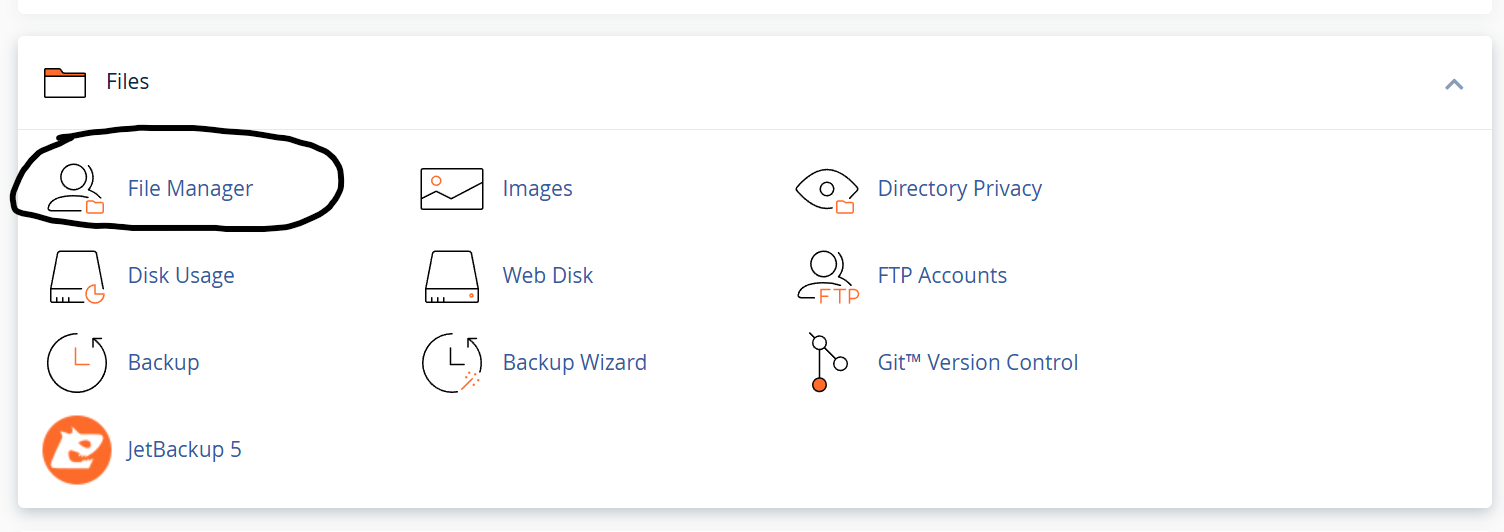
\includegraphics[width=10cm]{Gambar/bab3/instalasi-sistem-online/instalasi-sistem-online-tombol-file-manager.png}
    	\caption{Tombol \textit{Menu File Manager} Pada CPanel}
    	\label{fig:instalasi-sistem-online-tombol-menu-file-manager-pada-cpanel}
        \end{figure}
        \FloatBarrier
        \item Menekan tombol "\textit{Upload}" yang terdapat pada \textit{file manager} dan \textit{upload folder} aplikasi presensi \textit{online} yang telah di-\textit{zip} sebelumnya, serta melakukan \textit{extract} pada \textit{folder} tersebut. \textbf{\ref{fig:instalasi-sistem-online-tombol-tombol-upload-pada-file-manager}} menunjukkan tombol \textit{upload} pada \textit{file manager}.
        \begin{figure}[!htbp]
    	\centering
    	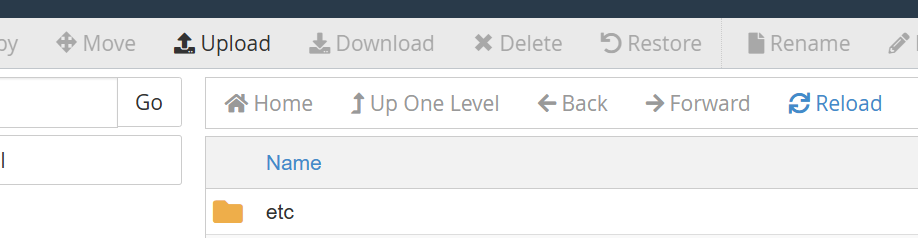
\includegraphics[width=10cm]{Gambar/bab3/instalasi-sistem-online/instalasi-sistem-online-tombol-upload-pada-file-manager.png}
    	\caption{Tombol Upload Pada \textit{File Manager}}
    	\label{fig:instalasi-sistem-online-tombol-tombol-upload-pada-file-manager}
        \end{figure}
        \FloatBarrier
    \end{enumerate}
    
    \item Memindahkan seluruh isi dari \textit{folder public} pada aplikasi presensi \textit{online} ke public\_html. \textbf{\ref{fig:instalasi-sistem-online-folder-public-html}} menunjukkan \textit{folder} public\_html pada \textit{file manager}.
    \begin{figure}[!htbp]
    	\centering
    	
\includegraphics[width=10cm]{Gambar/bab3/instalasi-sistem-online/instalasi-sistem-online-folder-public-html.png}
    	\caption{\textit{Folder} Public\_html Pada \textit{File Manager}}
    	\label{fig:instalasi-sistem-online-folder-public-html}
        \end{figure}
        \FloatBarrier

    \item Melakukan konfigurasi \textit{path} \textit{require} dan \textit{app} pada \textit{file} index.php yang terletak pada public\_html sebelumnya dengan nama \textit{folder} aplikasi presensi \textit{online}. \textbf{\ref{fig:instalasi-sistem-online-konfigurasi-file-index-php}} menunjukkan isi \textit{file} index.php yang telah dikonfigurasi.

    \begin{figure}[!htbp]
    	\centering
    	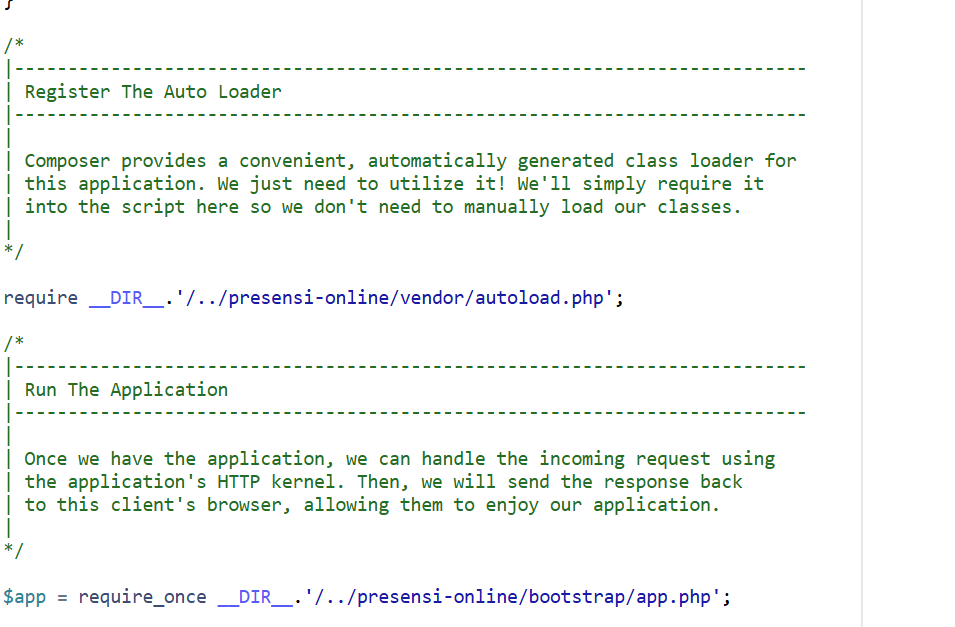
\includegraphics[width=10cm]{Gambar/bab3/instalasi-sistem-online/instalasi-sistem-online-konfigurasi-file-index-php.png}
    	\caption{Konfigurasi \textit{File} Index.php Pada Public\_html}
    	\label{fig:instalasi-sistem-online-konfigurasi-file-index-php}
        \end{figure}
        \FloatBarrier

    
    \item Melakukan konfigurasi pada \textit{file} .env untuk mengatur basis data dan mengatur \textit{email} yang akan digunakan untuk pengiriman kode OTP.
    
    \item Mengatur \textit{basis data} melalui menu PhpMyAdmin pada CPanel.
    \begin{enumerate}
        \item Menekan menu PHPMyAdmin pada CPanel. \textbf{\ref{fig:instalasi-sistem-online-tombol-phpmyadmin-pada-cpanel}} menunjukkan tombol PHPMyAdmin pada CPanel.
        \begin{figure}[!htbp]
    	\centering
    	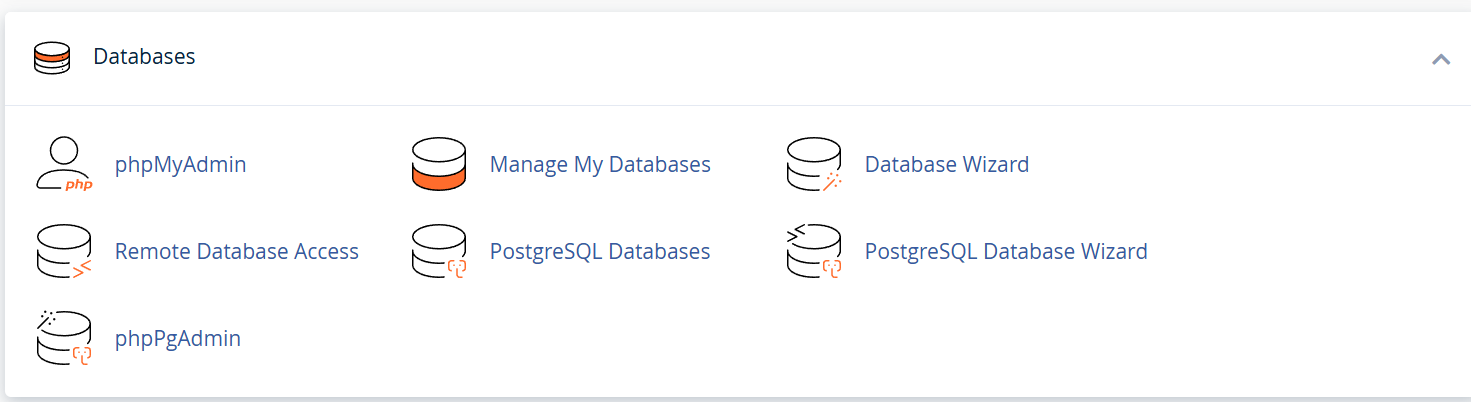
\includegraphics[width=10cm]{Gambar/bab3/instalasi-sistem-online/instalasi-sistem-online-tombol-phpmyadmin.png}
    	\caption{Tombol PHPMyAdmin Pada CPanel}
    	\label{fig:instalasi-sistem-online-tombol-phpmyadmin-pada-cpanel}
        \end{figure}
        \FloatBarrier
        \item Melakukan \textit{import file} .sql yang telah didapatkan melalui aplikasi presensi \textit{online} saat dijalankan secara lokal. \textbf{\ref{fig:instalasi-sistem-online-tombol-import-pada-cpanel}} menunjukkan tombol "\textit{Import}" pada PHPMyAdmin.
        \begin{figure}[!htbp]
    	\centering
    	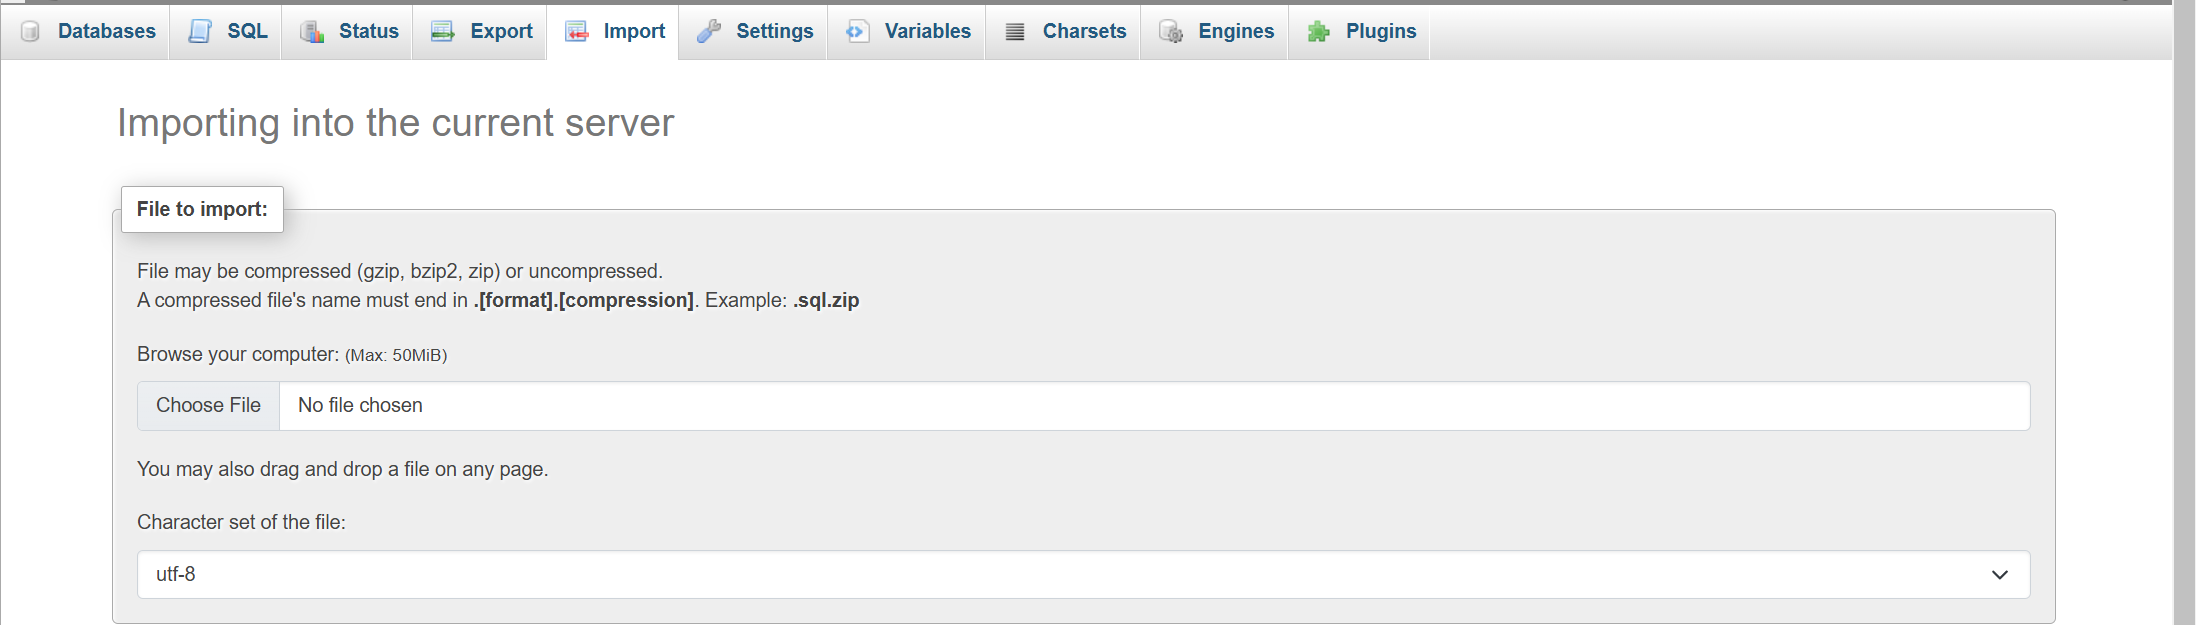
\includegraphics[width=10cm]{Gambar/bab3/instalasi-sistem-online/instalasi-sistem-online-tombol-import-phpmyadmin.png}
    	\caption{Tombol \textit{Import} Pada PHPMyAdmin}
    	\label{fig:instalasi-sistem-online-tombol-import-pada-cpanel}
        \end{figure}
        \FloatBarrier
    \end{enumerate}
    \item Melakukan instalasi SSL.
    \begin{enumerate}
        \item Menekan tombol menu \textit{"Let's Encrypt"} pada CPanel. \textbf{\ref{fig:instalasi-sistem-online-tombol-lets-encrypt}} menunjukkan tombol menu "\textit{Let's Encrypt}" pada CPanel.
        \begin{figure}[!htbp]
    	\centering
    	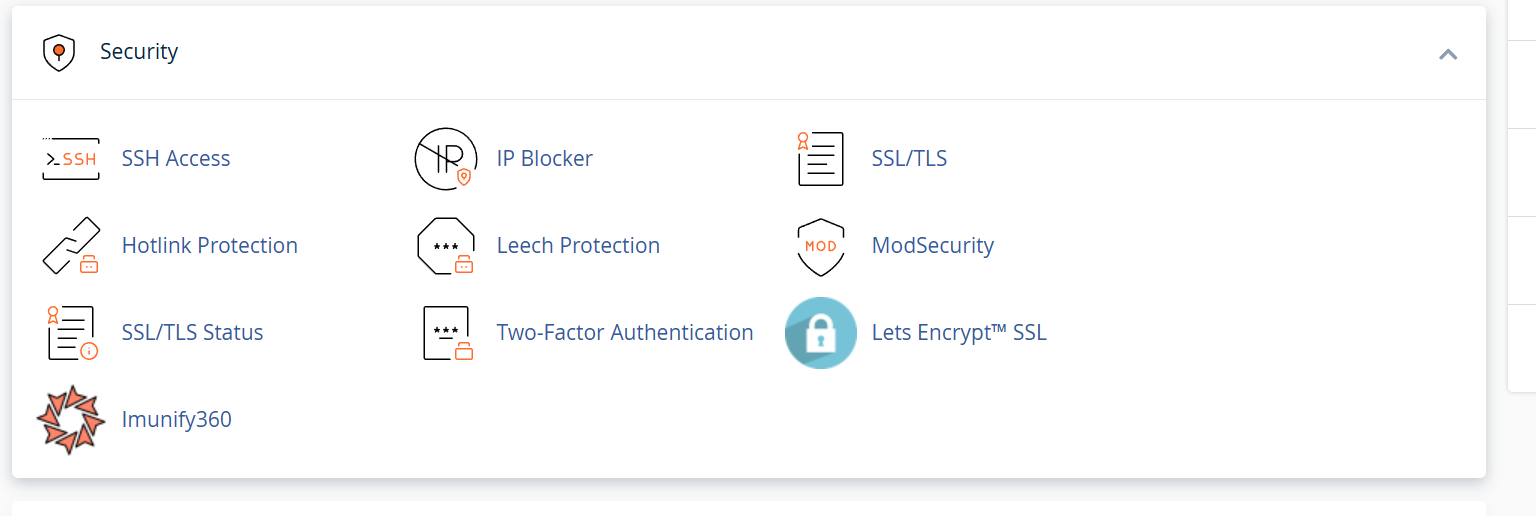
\includegraphics[width=10cm]{Gambar/bab3/instalasi-sistem-online/instalasi-sistem-online-tombol-lets-encrypt.png}
    	\caption{Tombol \textit{Let's Encrypt} Pada CPanel}
    	\label{fig:instalasi-sistem-online-tombol-lets-encrypt}
        \end{figure}
        \FloatBarrier
        \item Pada bagian \textit{Issue a new certificate}, tekan tombol "+ \textit{Issue}". \textbf{\ref{fig:instalasi-sistem-online-tombol-plus-issue-pada-lets-encrypt}} menunjukkan tombol "+ \textit{Issue}" pada bagian \textit{Issue a new certificate}.
        \begin{figure}[!htbp]
    	\centering
    	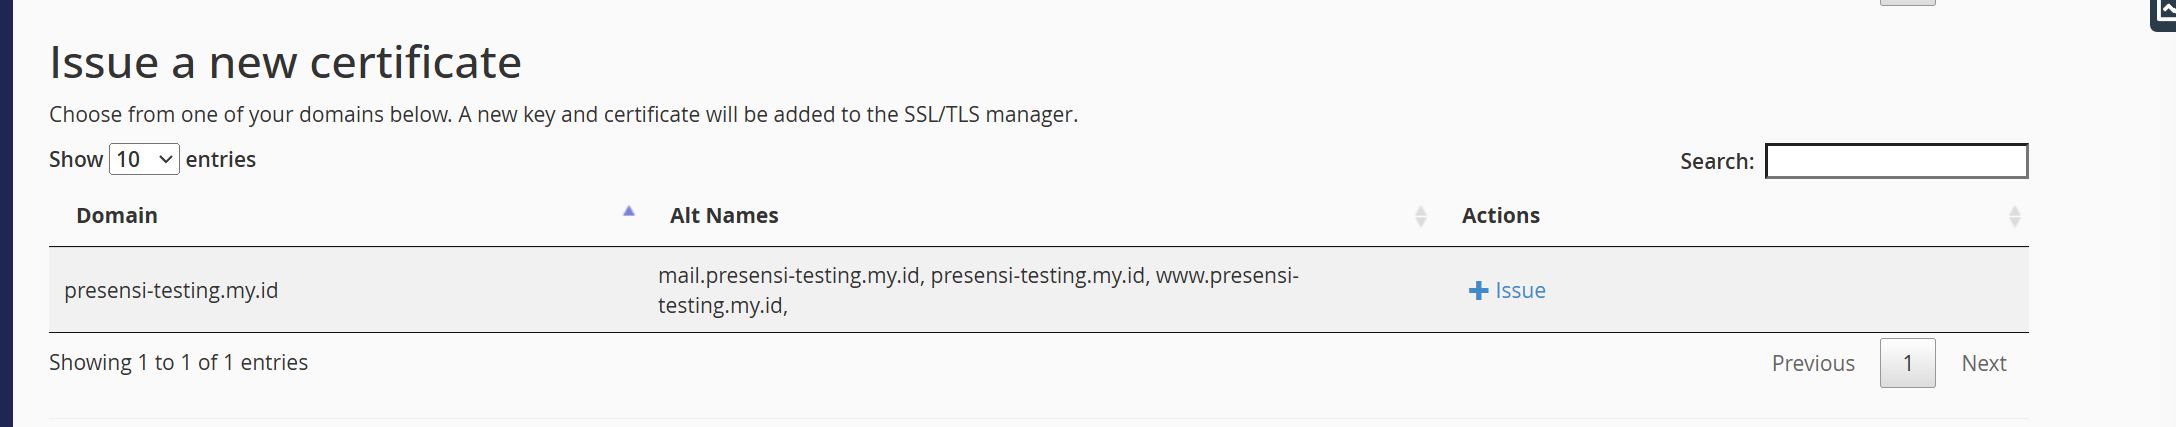
\includegraphics[width=10cm]{Gambar/bab3/instalasi-sistem-online/instalasi-sistem-online-tombol-issues-pada-lets-encrypt.png}
    	\caption{Tombol + \textit{Issue} Pada \textit{Let's Encrypt}}
    	\label{fig:instalasi-sistem-online-tombol-plus-issue-pada-lets-encrypt}
        \end{figure}
        \FloatBarrier
        \item pada bagian metode validasi SSL, pilih dns-01 dan tekan tombol "\textit{Issue}" untuk menyimpan metode yang dipilih. \textbf{\ref{fig:instalasi-sistem-online-tombol-dns01}} menunjukkan pilihan metode dns-01.
        \begin{figure}[!htbp]
    	\centering
    	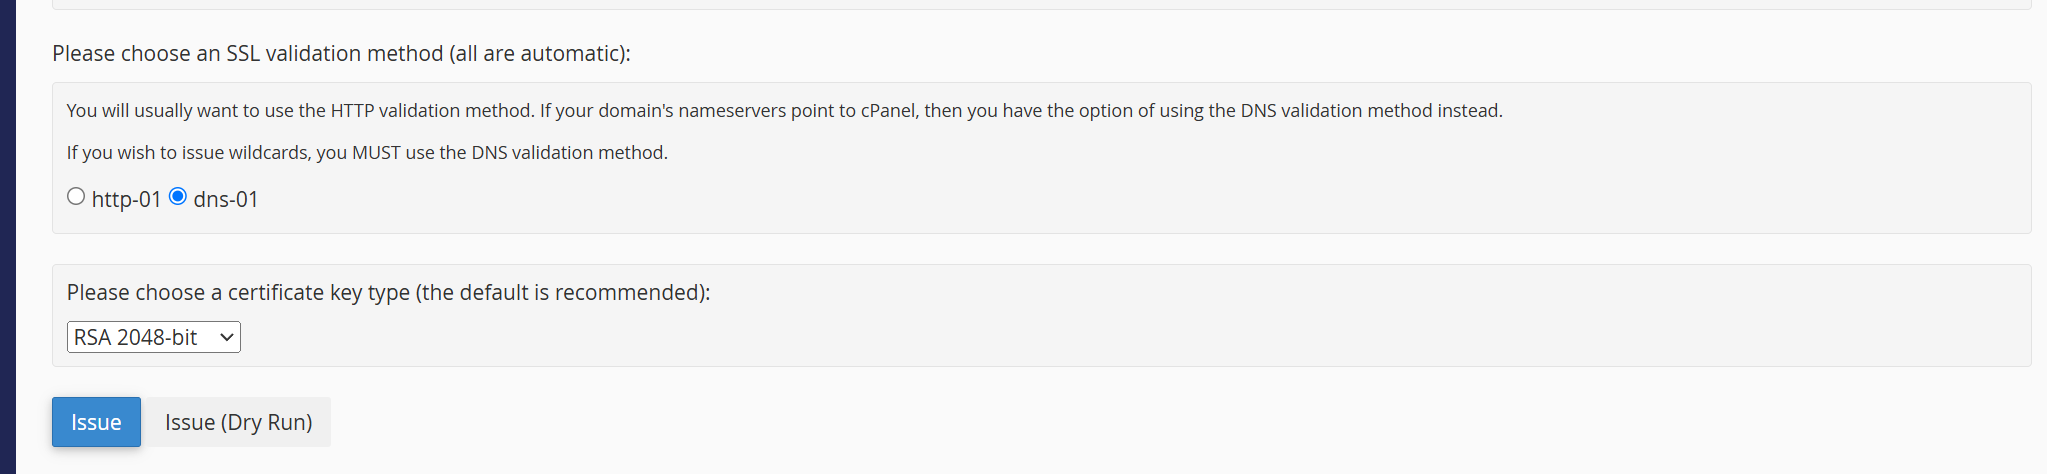
\includegraphics[width=10cm]{Gambar/bab3/instalasi-sistem-online/instalasi-sistem-online-tombol-dns01-pada-issues.png}
    	\caption{Metode Validasi SSL Dns-01}
    	\label{fig:instalasi-sistem-online-tombol-dns01}
        \end{figure}
        \FloatBarrier
    \end{enumerate}

\end{enumerate}

\subsection{\textit{User Manual}}
Terdapat \textit{user manual book} sebagai panduan untuk menggunakan aplikasi presensi \textit{online}. Pastikan telah melakukan instalasi sistem aplikasi secara lokal ataupun \textit{online} yang telah dilakukan pada \textbf{Subbab \ref{sec:instalation-system}} \textit{User manual book} dapat dilihat pada \textbf{\hyperref[sec:user-manual-aplikasi-presensi-online]{Lampiran~XII}}.
